\chapter{KRD(Kuantum Renk Dinamiği)}
Proton-Proton çarpışmasın da aslında çarpışma kuarklar ve gluonlar arasında gerçekleşir. Kuark ve gluonların özellikleri ve aralarındaki etkileşimleri KRD\footnote{Quantum chromodynamics } ile belirlenir. Bu bölümde kuarkların yapısı, asimptotik özgürlük, yükün perdelenmesi, korunum yasaları gibi konuların üzerinde durulacaktır. CMS deneyinde çıkan jetlerin\footnote{Bölüm 4.2 de anlatılacaktır } tanımlanması temelinde KRD önemli olduğu için bu konu üzerinde durulacaktır.
\par Bildiğimiz kadarıyla doğada dört temel kuvvet bulunmaktadır. Bunlar;
\begin{table}[!htbp]
\centering
\begin{tabular}{|c|c|c|c|}
\hline 
\textit{Kuvvet} & \textit{Şiddeti} & \textit{Kuram} & \textit{Aracı} \\ 
\hline 
Güçlü & 10 & Renk Dinamiği & Gluon \\ 
\hline 
Elektromanyetik & $10^-2$ & Elektrodinamik & Foton \\ 
\hline 
Zayıf & $10^-{13}$ & Çeşni dinamiği & W ve Z \\ 
\hline 
Kütleçekim & $10^{-42}$ & Geometrodinamik & Graviton \\ 
\hline 
\end{tabular} 
\caption{Doğada bulunan Kuvvetler, Şiddetleri ve Taşıyıcı Araçları}
\end{table}
\par Bu kuvvetlerin her birine bir parçacık değiş tokuşu aracılık etmektedir. Bu aracılar bir kuark veya bir lepton arasında kuvvet iletimini sağlarlar. Bu etkileşmeler belirli kurallar altında olmak zorundadırlar. Bunlardan birisi kuantum renk dinamiğidir.

\par Kuantum renk dinamiğinde, $renk$ yükün rolünü üstlenir ve temel süreç ($e \rightarrow e + \gamma$ sürecine benzeyen ) kuark $\rightarrow$ kuark + gluon $(q \rightarrow q + g)$\footnote{Leptonlar renk taşımadıkları için , güçlü etkileşmelere katılmazlar.}etkileşmesidir. 
\begin{figure}[!htbp]
\centering
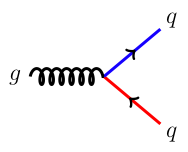
\includegraphics[scale=1]{quarkgluevertex.png}
\caption{Quark quark gluon etkileşimi}
\label{fig:quark}
\end{figure}
İki kuark arasındaki kuvvet en düşük mertebede Şekil \ref{fig:etkilesim} ile belirlenir.
\begin{figure}[!htbp]
\centering
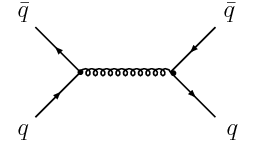
\includegraphics[scale=0.5]{qbarq-qbarq-scattering.png}
\caption{İki kuark arasındaki en düşük mertebeli etkileşim}
\label{fig:etkilesim}
\end{figure}
İki kuark arasındaki kuvvetin qluonların değiş-tokuşu ile taşındığı söylenebilir.
\par Bu düzeyde KRD, KED'e çok benzemektedir. Ancak önemli farklar da vardır. KED de tek bir elektrik yükü varken KRD'de $3$ çeşit rengin bulunmasıdır. $q \rightarrow q + g $ temel sürecinde kuarkın rengi değişebilir (fakat çeşnileri değişmez). Örneğin bir mavi yukarı-kuark, bir kırmızı yukarı-kuarka dönüşebilir. Renk Yükü her zaman korunur; bu, aradaki farklı gluonun taşıdığı anlamına gelir. Şekil \ref{fig:quark} da görüldüğü üzere kuarkların reklerinin biri mavi diğeri kırmızı olabilir bu durumda qluonun rengi $m , \overline{k}$ dır ve renk yükü korunmuş olur. Böylece qluonun iki renkli olduğu anlaşılmaktadır.
\par Gluonların kendileri renk taşıdıkları için doğrudan diğer gluonlarla etkileşmeye girerler, dolayasıyla ilkel kuark-gluon köşesinde ilave olarak ilkel gluon-gluon köşesi vardır.
\begin{figure}[!htbp]
\centering
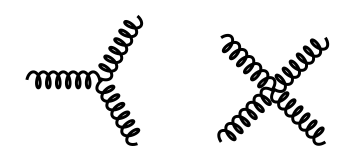
\includegraphics[scale=1]{WorldOfGlue.png}
\caption{İki çeşit gluon etkileşmesi; 3 gluon köşesi ve dörk gluon köşesi}
\end{figure}
Bu doğrudan gluon-gluon çiftlenimi, KRD'ni KED`e göre daha karmaşık fakat aynı zamanda çok daha zengin kılar.
\par Renk dinamiği ile elektrodinamiği arasında diğer bir fark da çiftlenim sabitinin büyüklüğüdür. KED`ğinde her köşe, hesaba $\alpha =1/137$ faktörü katar. Bu sayının küçük olmasının anlamı, sadece az sayıda köşeye sahip Feynman diyagramlarını göz önüne almamızın yeterli olmasıdır. Güçlü kuvvetler için karşılık gelen çiftlein sabiti $\alpha_s$ 1 den büyük olduğu deneysel olarak gösterilmiştir.
\par Daha karmaşık diyagramlar daha çok katkıda bulunmaktadırlar ve KED için çok iyi çalışan Feynman diyagramları bu durumda işe yaramamaktadırlar. Kuantum renk dinamiğinin büyük zaferlerinin birisi, bu kuramda çiftlenim sabiti rolü oynayan sayının aslında bir sabit olmayıp etkileşen parçacıklar arasındaki uzaklığa bağlı olduğunun keşfidir.\footnote{kayan çiftlenim sabiti.} Nükleer fiziğin karakteristiği olan nispeten uzun mesafelerde büyük iken, çok kısa mesafelerde çok küçük değerler alır. Bu olaya Asimptotik özgürlük olarak bilinir. Asimptotik özgürlük daha net bir deyişle bir proton veya bir pionun içinde kuarkların birbirleriyle fazla etkileşmeden bir arada durmasıdır. Bu davranış deneysel olarak derin esnek olmaya saçılma deneylerinde gözlenmiştir. Kuramsal bakış açısından, asimptotik özgürlüğün keşfedilmesi, yüksek enerjide Feynman cebrinin KRD için geçerli hesaplama aracı olmasını sağlamıştır.

\begin{figure}[!htbp]
\centering
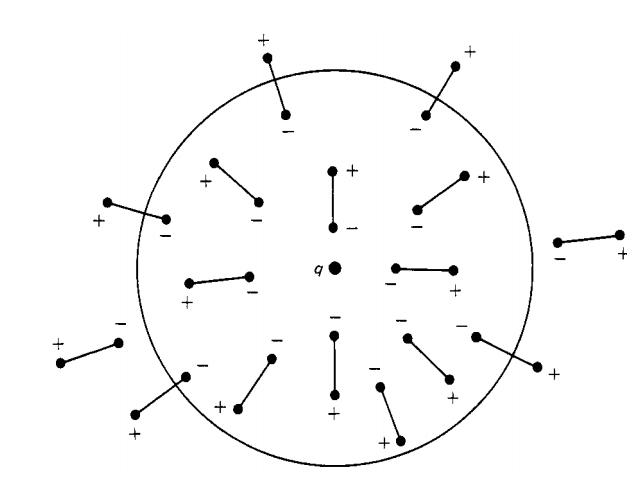
\includegraphics[scale=0.4]{qyuku.png}
\caption{dielektrik bir ortamda bir q yükünün perdelenmesi}
\label{fig:qyuku}
\end{figure}
\par Elektrodinamikte etkin çiftlenim sabiti, kaynaktan olan uzaklığımıza bağlıdır. Bu, nicel olarak şu şekilde anlaşılabilir. İlk olarak bir dielektrik ortam içinde gömülü bir pozitif noktasal q yükünü göz önüne alalım. Şekil \ref{fig:qyuku} 'de gösterildiği gibi, her moleküler dipolün negatif ucu q`ya doğru çekilir ve pozitif ucu uzağa itilir. Sonuç olarak parçacık etrafında, alanı kısmen iptal eden negatif yüklerden oluşan bir kaplama oluşur. Dolayısı ile dielektrik ortamın varlığında, herhangi bir parçacığın etkin yükü bir miktar indirgenir. Tabii ki en yakın molekülden daha yakındaysanız perdeleme yoktur ve q yükünün tümünü görürsünüz.Etkin yük çok küçük uzaklıklarda artmış olur.
\par Kuantum elektrodinamiğinde vakımın kendisi tıpkı bir dielektrik madde gibi davranır. Şekil \ref{fig:feyndiyagram} da gösterildiği gibi pozitron-elektron çiftleri oluşturur.
\begin{figure}[!htbp]
\centering
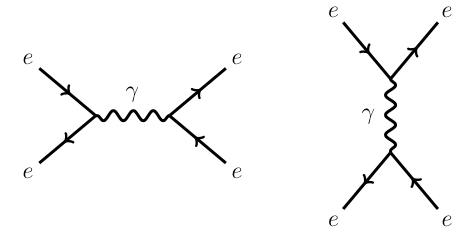
\includegraphics[scale=0.8]{feyndiyagram.png}
\caption{elektron pozitron çiftleri}
\label{fig:feyndiyagram}
\end{figure}

\par Halka sanal elektron q'ya doğru çekilir ve sana pozitron uzağa itilir bu şekilde ortaya çıkan vakum kutuplanması yükü kısmen perdeler ve alanı azaltır. Bir kez daha q yüküne çok yaklaşılırsa perdeleme kaybolur. Her zaman elektron yükü olarak adlandırdığımız büyüklük aslında tümüyle perdelenmiş etkin yüktür. KED`ğindeki durum böyledir. Aynı durum KRD'de de söz konusudur.kuark-kuark-gluon köşesinin yanı sıra şimdi doğrudan gluon-gluon köşeleride vardır.KED`deki vakum kutuplanabilirliğine benzeyen diyagramlara ek olarak şimdi gluon halkalarının da hesaba katmalıyız.
\begin{figure}[!htbp]
\centering
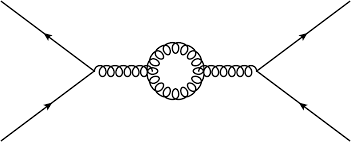
\includegraphics[scale=0.5]{gluonloop.png}
\caption{Gluon loop a sahip bir feynman diyagramı}
\label{fig:gluonloop}
\end{figure}
kuark kutuplanma diyagramları (bunlar kısa mesafelerde $\alpha_s$'yi yukarıya çeker) ile gluon kutuplanması (bunlar ise aşağıya çeker) arasında bir çeşit yarış vardır.

\begin{equation}
a\equiv 2f - 11 n
\end{equation}
Bu sayı pozitif ise, KED`de olduğu gibi etkin çiftlenim kısa mesafelerde artar; negatif ise azalır. Standart Model'de $f=6$ ve $n=3$ ve $a=-21$'dir ve KRD çiftlenimi kısamesafelerde azalır. Asimptotik özgürlüğün kaynağı budur.

\section{Zayıf Etkileşmeler}
elektriksel yükün elektromanyetik kuvvetleri ve renk yükünün güçlü kuvveti üretmesi anlamında zayıf kuvvetleri üreten şeyin özel bir adı yoktur.Tüm kuarklar ve leptonlar bu yükü taşımaktadırlar. İki tür zayıf etkileşme söz konusudur. Bunlar yüklü etkileşmeler (W ların aracılık yaptığı) ve yüksüz etkileşmelerdir(Z'nin aracılık yaptığı).
\subsection{Yüksüz Zayıf Etkileşim}
Z bozonu nötrino-proton saçılması gibi süreçlere aracılık eder.
\begin{figure}[!htbp]
\centering
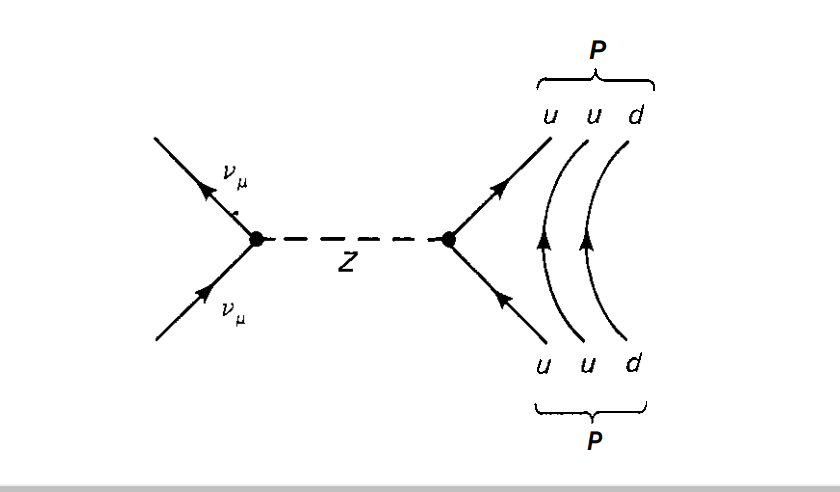
\includegraphics[scale=0.3]{yuksuzZ.png}
\caption{yüksüz etkileşim örneği olarak feynman diyagramı}
\end{figure}
Son durum da,d'ye güçlü kuvvetlerle (gluon değiş tokuşu) bağlı olan  iki seyirci kuark aktif rol oynamadan olaya katılır. Bir fotonun aracılık ettiği herhangi bir sürece Z'nin de aracılık edebilebilir. Coulomb yasasına ikinci diyagramdan gelen bir düzeltme vardır fakat fotonun aracılık yaptığı süreç çok baskındır. Atom fiziğinde, elektromanyetik süreçlerdeki yüksüz zayıf kirlilik zayıf etkileşmelerin taşıdığı parmak izinden yararlanılarak ayırt edilebilir. Katkının çok küçük olmasından dolayı nötrino deneyleri oldukça zordur.
\subsection{Yüklü Zayıf Etkileşim}
İlkel köşelerin güçlü, elektromanyetik ve yüksüz zayıf etkileşimler için paylaşıldığı özellik, çıkan kuark veya leptonun gelen ile aynı olmasıdır. KRD'de kuarkların rengi değişebilir ama çeşni hiçbir zaman değişmez. Çeşniyi değiştiren sadece yüklü zayıf etkileşmelerdir.
\subsubsection{Leptonların Yüklü Zayıf Etkileşimi}
Bir negatif yüklü lepton bir $W^-$ yayımlayarak buna karşılık gelen bir nötrinoya dönüşür. 
\begin{figure}[!htpb]
\centering
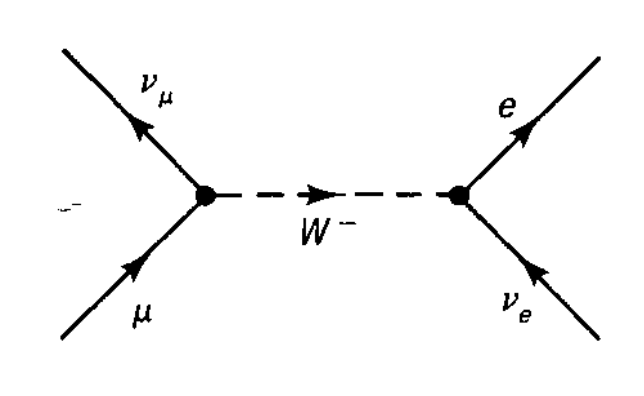
\includegraphics[scale=0.3]{leptonlar.png}
\caption{Leptonik bozunum}
\end{figure}


\subsection{Kuarkların Etkileşimi}
Bu kuram da elektron sayısı, müon sayısı ve tau sayısının korunumu şattır. Şekil \ref{fig:cesnidegis} 'de $-1/3$ yüklü bir kuark bir $W^-$ bozonu yayımlayarak $+2/3$ yüklü bir kuarka dönüşür. Çıkan kuark gelen kuarkla ayrı rengi taşır, ama çeşnisi değişmiştir.

\begin{figure}[!htpb]
\centering
\begin{subfigure}{.5\textwidth}
  \centering
  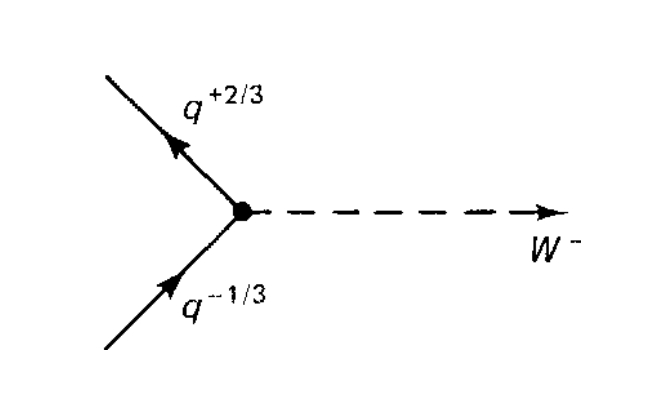
\includegraphics[width=.8\linewidth]{cesnidegis.png}
  \caption{$W^-$ ozunumuyla çeşni değiştiren quarklar}
  \label{fig:cesnidegis}
\end{subfigure}%
\begin{subfigure}{.5\textwidth}
  \centering
  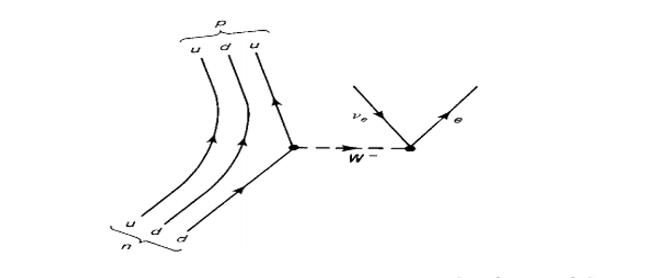
\includegraphics[width=.8\linewidth]{protonnotron.png}
  \caption{Nötronun beta bozunumu}
  \label{fig:sub2}
\end{subfigure}
\caption{Kuark etkileşmesi}
\label{fig:test}
\end{figure}

Bu etkileşim ile temelde nötronun beta bozunumunu da gösterebiliriz.

\subsection{Bozunumlar ve Korunum Yasaları}
Temel parçacıkların en genel özelliklerinden birisi parçalanmaya olan eğilimleridir. Bu durumu evrensel bir ilke şeklinde ifade edebiliriz. Bir korunum yasası tarafından engellenmediği sürece, her parçacık kendisinden daha hafif parçacıklara bozunur.
\begin{table}[!htpb]

\centering
\begin{tabular}{|c|c|c|}
\hline 
foton & kararlı & kütlesiz \\ 
\hline 
elektron & kararlı & en hafif yüklü parçacık \\ 
\hline 
proton & kararlı & en hafif baryon \\ 
\hline 
\end{tabular}
\caption{bazı parçacıkların kararlılıkları ve sebebleri}
\end{table}
Tablo  da açıkça görüldüğü üzere yük korunumu ve baryon korunumu için bu temel parçacıklar için kararlı diyebiliyoruz.Fakat çoğu parçacık (birçok atom çekirdeğinin koruyucu ortamında kararlı olmakla birlikte nötron bile) kendiliğinden bozunur.Çevremizde esas olarak protonlar, nötronlar, elektronlar, fotonlar ve nötrinolar bulunmaktadır. Daha egzotik parçacıklar zaman zaman çarpışmalarda üretilirler ama fazla yaşamazlar.Her kararsız türün bir karakteristik ömrü $\tau$ vardır. Parçacıkların çoğu birkaç farklı bozunum moduna sahiptir, örneğin $K^+$ ların $\%64$ ü $(\mu^+ + v_\mu )$ şeklinde bozunurken, $\%21$'i $(\pi^+ + \pi^0)$'a $\%6$'sı $(\pi^+ + \pi^+ + \pi^- )$'ye ve $\%5$'i ise $(e^+ + v_e + \pi^0)$'a bozunmaktadır. Temel parçacık kuramının hedeflerinden birisi de bu ömür ve dallanma oranlarının hesaplanmasıdır. 
\par Verilen bir bozunum üç temel kuvvetten birisi tarafından meydana getirilir. Bunlar güçlü, elektromanyetik ve ya zayıf boozunumlardır.

\begin{table}[!htpb]
\centering
\begin{tabular}{|c|c|}
\hline 
Bozunum & Bozunum Türü \\ 
\hline 
$\triangle^{++} \rightarrow p^+ + \pi^+$ & Güçlü  \\ 
\hline 
$\pi^0 \rightarrow \gamma + \gamma$ & Elektromanyetik \\ 
\hline 
$\sum^- \rightarrow n + e^- + \overline{v_e} $ & Zayıf \\ 
\hline 
\end{tabular} 

\caption{Bozunumlar ve Bozunum Türleri}
\end{table}
Eğer bozunumda bir foton çıkıyorsa süreç mutlaka elektromanyetik, nötrino çıkıyorsa mutlaka zayıftır. Ancak bunlar çıkmadığında ne olduğunu söylemek oldukça zordur. Güçlü bozunumun ömrü $10^{-23}s$ civarında, elektromanyetik bozunum  $10^{-16}s$ ve zayıf bozunum $10^{-13}s$'den 15 dakikaya kadar değişebilir.Bozunum genellikle ana parçacık ile ürün parçacık arasındaki kütle farkıyla ters orantılıdır.  

\begin{figure}[!htpb]
\centering
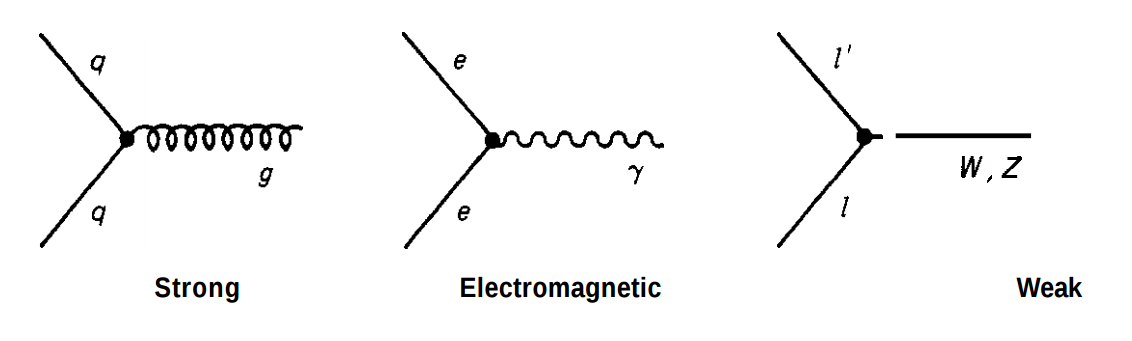
\includegraphics[scale=0.4]{bozunumkurallari.png}
\caption{üç bozunum türü için Feynman diyagramları}
\end{figure}
Tüm fiziksel süreçleri temel diyagramları karmaşık kombinasyonlar halinde bir araya getirerek elde etmek mümkün olduğundan dolayı, her köşe için tepkimenin tamamında korunmalıdır. Korunma yasaları;

\begin{enumerate}
\item \emph{Yük : } 
\par Her üç etkileşmedede elektrik yükünü korur. Zayıf etkileşmelerde yük farkı olabilir ve bu farkı W taşır.
\item \emph{Renk : }
\par Elektromanyetik ve zayıf etkilşmelerde renk etkilenmez. Bir güçlü etkileşim köşesinde kuark rengi değişir, farkı gluon taşır.Doğada bulunan parçacıklar renksiz olduğundan korunumun gözlenmesi çok kaydır. Tepkimeye giren renk sıfır ve tepkimeden çıkan renk sıfır olmalıdır.

\item \emph{Baryon Sayısı : }
\par Bütün ilkel köşelerde, eğer bir kuark girerse, bir kuark da çıkar ve dolayısı ile mevcut kuark sayısı sabittir. Bu işlem de antikuarklar negatif sayılır.

\item \emph{Lepton Sayısı : }
\par Güçlü kuvvetler hiç bir şekilde leptonlara dokunmaz; bir elektromanyetik etkileşmede giren lepton aynen çıkar.

\item \emph{Çeşni : }
\par Çeşni güçlü ve elektromanyetik köşelerde korunur ancak zayıf etkileşim köşelerinde korunmaz.Yani bir yukarı kuark bir aşağı-kuark veya acayip kuarka dönüşebilir.Kaybedilen yukarılığı taşıyan veya kazanılan aşağılığı veya acayipliği sağlayan birşey yoktur. Zayıf kuvvetler çok zayıf olduğundan değişik çeşnilerin yaklaşık olarak korunduğunu söyleriz.

\end{enumerate}
